% Chapter Template

\chapter{PubSeq Solr Index} % Main chapter title

\label{Chapter5} % Change X to a consecutive number; for referencing this chapter elsewhere, use \ref{ChapterX}

\lhead{Chapter 5. \emph{PubSeq Solr Index}} % Change X to a consecutive number; this is for the header on each page - perhaps a shortened title

This chapter tries to answer the second question posed in Section \ref{sec:Chap3Intro}: \textit{how the data is going to be stored?} We would see the reason behind our choice of storage technology. We would then also try to specify the definition of our index.

%----------------------------------------------------------------------------------------
%	SECTION 1
%----------------------------------------------------------------------------------------

\section{Solr: Fast and Scalable Indexing}

Apache Solr is an open source enterprise search platform. Initially developed by Yonik Seeley at CNET Networks, it was later published as open source through donation to Apache Software Foundation \footnote{\href{https://issues.apache.org/jira/browse/SOLR-1}{\texttt{https://issues.apache.org/jira/browse/SOLR-1}}, accessed 25/08/2015}. The system is based on Lucene internally, which implements the indexing routine and mechanism \citep{hatcher2004lucene}.

Unlike SQL based system which uses tabular data representation as underlying data storage mechanism, Solr utilizes indexing mechanism in its system \citep{smiley2015apache}. This non-SQL characteristics of data storage and maintenance are generally known as NoSQL. (Brewer, 2000) \citep{brewer2000towards} did some nice overview of comparison between NoSQL and conventional SQL, which could be seen on Table \ref{fig:ACIDvsBASE}

\begin{table}[htbp]
\caption{ACID vs. BASE database property models.}{ACID vs. BASE database property models. Some NoSQL databases implement ACID, others do not. Taken from (Wachinger, 2013) \citep{wachinger2013next}, adopted from (Brewer, 2000) \citep{brewer2000towards}.
}
\begin{tabularx}{\textwidth}{ | l | X | }
  \hline
  ACID (relational model) & BASE (NoSQL) \\
  \hline
  Atomicity, Consistency, Isolation, Durability & Basically Available, Soft state, Eventually consistent \\
  Isolation & Availability First \\
  Focus on Commit & Best Effort \\
  Nested Transactions & Approximative Answers Acceptable \\
  Non-quaranteed Availability & Aggressive (Optimistic) \\
  Conservative (pessimistic) & Simpler \\
  Difficult Evolution (schema) & Faster, Easier Evolution \\
  \hline
\end{tabularx}
  \label{fig:ACIDvsBASE}
\end{table}

While most NoSQL implementations don't strictly follow ACID criterions, most don't fall into BASE category either. Also, many NoSQL implementations focus on particular use case rather than aim at general data storage purpose. In this regard, Solr aims to be able to store and index in the order of millions and billions documents while optimizing for -- among others -- faceted search \citep{tunkelang2009faceted}, string search and result paging\footnote{\href{https://cwiki.apache.org/confluence/display/solr/Pagination+of+Results}{\texttt{https://cwiki.apache.org/confluence/display/solr/Pagination+of+Results}}, accessed 24/05/2015}. Solr also supports implicit definition of text syntax through definition of stopping sign, language rules etc -- this malleability is used for example, for Solr to be able to optimize for specific language it indexes \citep{grainger2014solr}. This way, Solr not only stores the data efficiently but in a way understand the logic of the data.

Formally, we define our reason of using Solr as follows:

\begin{itemize}
\item \textbf{Reverse indexing}. Possibly the strongest proposition of using Solr, reverse indexing refers to listing down \textit{where in which documents does a string appears in the index}, instead of \textit{which strings appear in which document in the index} \ref{fig:SolrReverseIndexing}. This reverse paradigm enables Solr to retrieve string related queries in almost constant time \citep{grainger2014solr}.
\item \textbf{Automatic Query Weighting}. In its query syntax, Solr enables weighted string matching query. Take for example following content of Solr query: 
\begin{center}
\texttt{unirotid:P53\_HUMAN\textasciicircum2 AND uniprotid:P53\_HORSE}
\end{center}
In this query, \texttt{unirotid:P53\_HUMAN} would be given twice as much weight as \texttt{uniprotid:P53\_HORSE}. For complex analysis involving multiple string queries this proves to be a powerful feature.
\item \textbf{Easy Deployment}. Each unpacked Solr directory could be run to create an instance of server. The only external requirement for Solr is installed Java Virtual Machine (JVM). This makes easier for us for example to test our index in various environment, therefore reducing iteration overhead.
\item \textbf{Native Java Implementation}. Combined with its native Java API, SolrJ, it ensures easier interaction and development of the index.
\item \textbf{Result Pagination}. Solr natively supports results pagination\footnote{\href{https://cwiki.apache.org/confluence/display/solr/Pagination+of+Results}{\texttt{https://cwiki.apache.org/confluence/display/solr/Pagination+of+Results}}, accessed 25/08/2015}. This means that, for very huge query result the system doesn't have to dump the whole result in memory. For our specific purpose, this proves helpful.
\end{itemize}

\begin{figure}[htbp]
    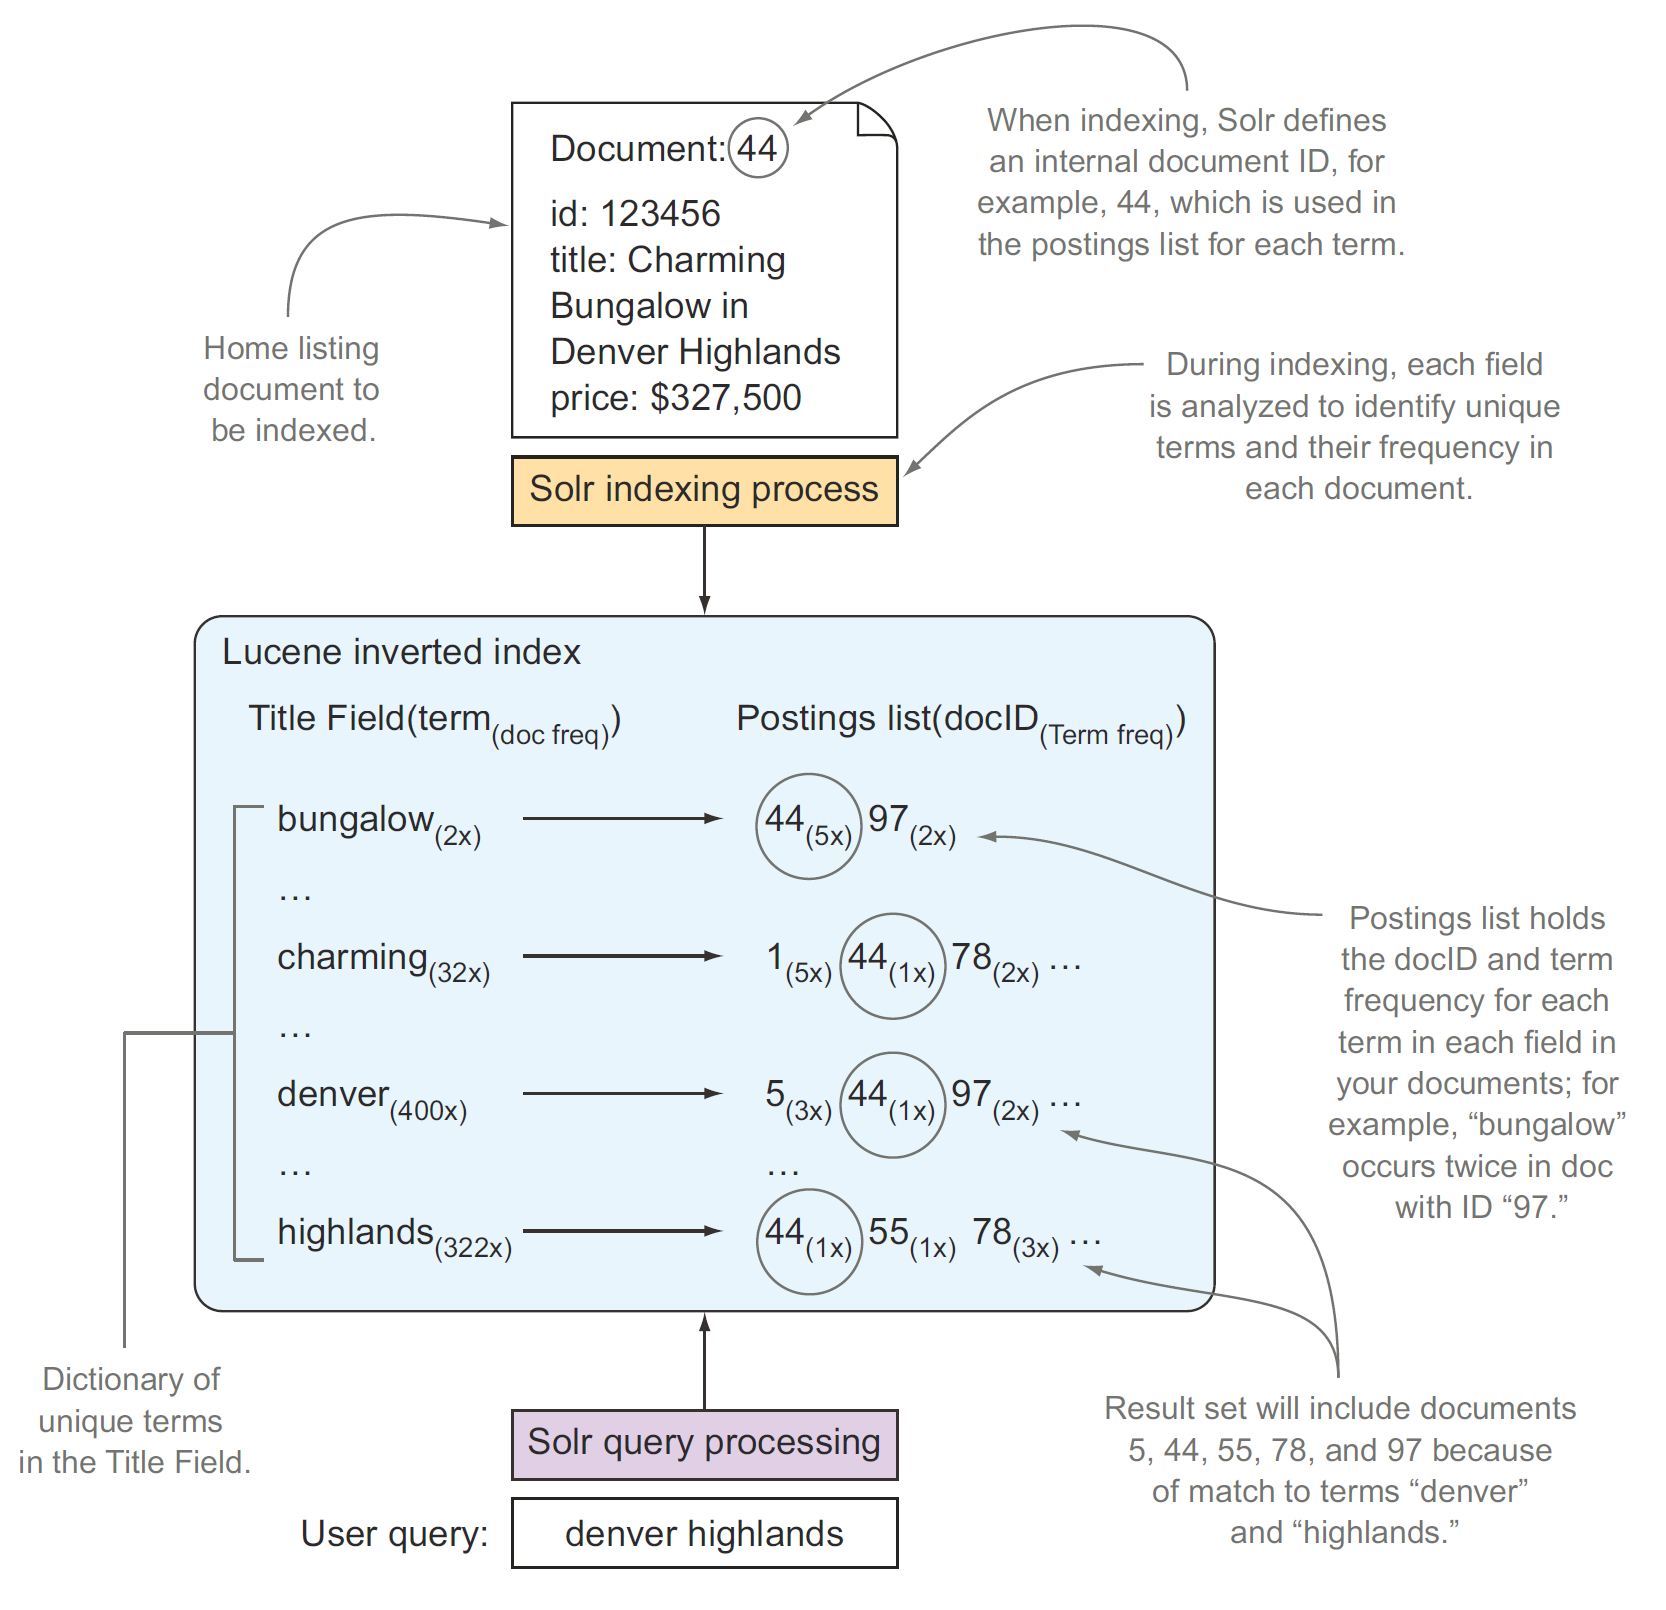
\includegraphics[width=6in]{Figures/solr_reverse_indexing.png}
    \rule{35em}{0.5pt}
  \caption[The key data structure supporting information retrieval is the inverted index within Solr system.]{Overview of reverse indexing mechanism employed by Solr. Here we see how a document is being parsed and represented internally within the mapping of tokens. Beyond Solr, reverese indexing is powerful tool in the field of Information Retrieval (IR) which enables finding occurrences in much reduced time \citep{manning2008introduction}. The fundamentals of reverse indexing in IR follows roughly the same concepts of Solr's reverse indexing. Figure adopted from (Grainger, Potter and Seeley, 2014 \citep{grainger2014solr})}
  \label{fig:SolrReverseIndexing}
\end{figure}

\begin{figure}[htbp]
    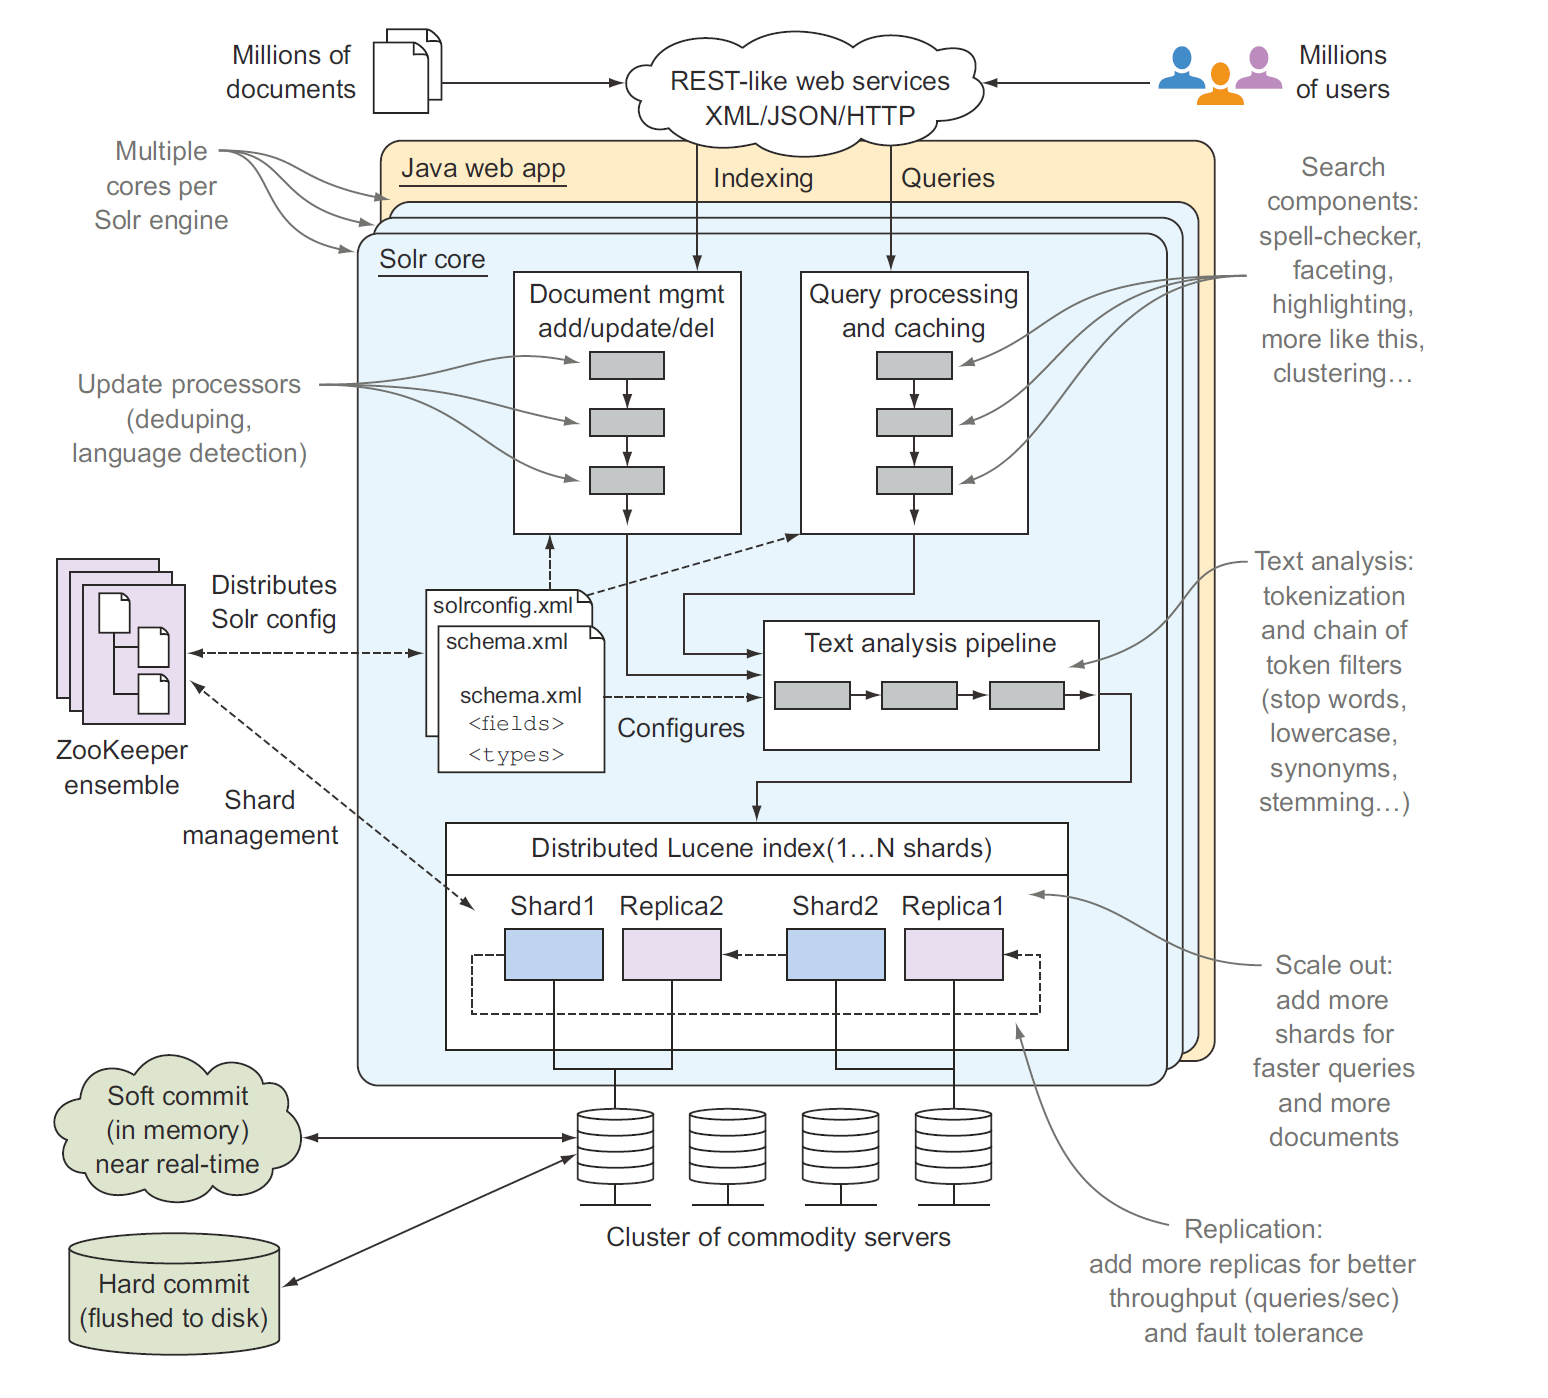
\includegraphics[width=6in]{Figures/solr_components.png}
    \rule{35em}{0.5pt}
  \caption[Diagram of the main components of Solr.]{Diagram of the main components of Solr. There are two main modes of index access: query and indexing. Both modes are handled by the top level REST-like service (wrapped in Jetty \citep{jetty}, Tomcat \citep{apachetomcat} or something similar). Each instance consists of multiple core, with each core is defined by configuration files, namely \texttt{solrconfig.xml} (which applies globally across all cores) and \texttt{schema.xml}. Both indexing and query routines would be going through text analysis pipeline for tokenization and other lexical analysis. Solr would then store/fetch several meta-information in/from appropriate Lucene index. Figure adopted from (Grainger, Potter and Seeley, 2014 \citep{grainger2014solr})}
  \label{fig:SolrComponents}
\end{figure}


There are also other reasons for deploying Solr such as generally lower schema definition complexity, generally powerful syntax etc., which makes even more case for using Solr over other both SQL and non-SQL systems.

%----------------------------------------------------------------------------------------
%	SECTION 2
%----------------------------------------------------------------------------------------

\section{Index Definitions}

Each Solr engine consists of several \textbf{cores} (see Figure \ref{fig:SolrComponents}). Solr wiki page wrote following regarding Solr Core \footnote{\href{https://wiki.apache.org/solr/SolrTerminology}{\texttt{https://wiki.apache.org/solr/SolrTerminology}}, accessed 25/08/2015}:

``
\textit{Solr Core: Also referred to as just a "Core". This is a running instance of a Lucene index along with all the Solr configuration (\texttt{SolrConfigXml}, \texttt{SchemaXml}, etc...) required to use it. A single Solr application can contain 0 or more cores which are run largely in isolation but can communicate with each other if necessary via the \texttt{CoreContainer}. From a historical perspective: Solr initially only supported one index, and the \texttt{SolrCore} class was a singleton for coordinating the low-level functionality at the "core" of Solr. When support was added for creating and managing multiple Cores on the fly, the class was refactored to no longer be a Singleton, but the name stuck.} 
``

Needless to say, Solr core is the lowest abstraction that is configurable within Solr environment. Each Solr core is defined by its own schema. In the mode we were running our Solr on\footnote{Depending on which Solr one is running, a schema could be defined either by \texttt{schema.xml} file or through Schema API (see here: \href{https://cwiki.apache.org/confluence/display/solr/Schema+API}{\texttt{https://cwiki.apache.org/confluence/display/solr/Schema+API}}, accessed 25/08/2015). Both interfaces trigger approximately the same configuration internally.}, we utilize \texttt{schema.xml} to define our schema. For someone more familiar in SQL-based lingo, a core could be thought analogously as table and schema its definition. This definition only works so far since communicating between two cores within Solr is not as trivial as it would be the case for tables in SQL environment.

Similar to SQL fashion, one of the most important aspect of schema definition within Solr is fields definition. We first define our fields in following table:

\begin{table}[htbp]
\caption{Fields definition table for \texttt{pubseq} index within the Solr system.}
\centering
\begin{tabular}{| l | c | c | c | c | c |}
  \hline
  name & type & indexed & stored & required & multiValued \\
  \hline
  \hline
  title & text\_general & \texttt{True} & \texttt{True} & \texttt{True} & \texttt{False} \\
  \hline
  abstract & text\_general & \texttt{True} & \texttt{True} & \texttt{False} & \texttt{False} \\
  \hline
  authors & text\_general & \texttt{True} & \texttt{True} & \texttt{False} & \texttt{True} \\
  \hline
  journal & text\_general & \texttt{True} & \texttt{True} & \texttt{True} & \texttt{False} \\
  \hline
  uniprotid & text\_general & \texttt{True} & \texttt{True} & \texttt{False} & \texttt{True} \\
  \hline
  speceisid & text\_general & \texttt{True} & \texttt{True} & \texttt{False} & \texttt{True} \\
  \hline
  meshid & text\_general & \texttt{True} & \texttt{True} & \texttt{False} & \texttt{True} \\
  \hline
\end{tabular}
  \label{fig:ACIDvsBASE}
\end{table}

\textbf{type} refers to what kind of Java class this field implements. If \textbf{indexed} is true, the value of the field can be used in queries to retrieve matching documents. If \textbf{stored} is true, the actual value of the field can be retrieved by queries. if \textbf{required} is true, the core instructs Solr to reject any attempts to add a document which does not have a value for this field. If \textbf{multiValued} is true, it indicates that a single document might contain multiple values for this field type\footnote{\href{https://cwiki.apache.org/confluence/display/solr/Defining+Fields}{\texttt{https://cwiki.apache.org/confluence/display/solr/Defining+Fields}}, accessed 25/08/2015}. Each multi-valued entry is represented as list internally. This could be invoked using any class implementing List interface \footnote{\href{http://docs.oracle.com/javase/7/docs/api/java/util/List.html}{\texttt{http://docs.oracle.com/javase/7/docs/api/java/util/List.html}}, accessed 25-08-2015}. As query result, depending on the return format (XML, JSON or CSV), this would be returned as either XML list, JSON list oobject or CSV cell-internal list respectively.

Upon creatoin of core, this configuration would be internalized via \texttt{schema.xml}. An example of instance of \texttt{schema.xml} can be found in Appendix \ref{sec:SchemaXMLPath}.

Following is a slightly redacted example of a document within Solr, which is taken for the paper by Karapakis-Liaskos and Ferrero, Nat. Rev. Immunol., 2015\footnote{doi:10.1038/nri3837}:

\label{lst:MEDLINEDTD}